Dotychczas zakładaliśmy, że granice między ośrodkami tworzącymi wielowarstwę są idealnie płaskie. W warunkach eksperymentalnych, przy wykorzystaniu technik umożliwiających naprzemienne układanie kilkunastu warstw różnych materiałów o~grubości od kilkunastu do kilkudziesięciu nanometrów,  takich jak fizyczne osadzanie z~fazy gazowej (ang.~PVD - physical vapour deposition), uzyskanie doskonale gładkich warstw jest niemożliwe. W poniższym rozdziale przeanalizowany zostanie wpływ niedoskonałości warstw na obrazowanie przez struktury MDM(metal-dielektryk-metal).

Podstawowym parametrem wykorzystywanym do opisu chropowatości jest średnia kwadratowa różnic faktycznej grubości warstwy od średniej (ang.~RMS - root mean square), wyrażana wzorem:
\begin{equation}
\textrm{RMS}=\sqrt{\sum_i^n \frac{(x_i -x_0)^2}{n}},
\end{equation}
gdzie $x_i$ są kolejnymi zmierzonymi grubościami, $x_0$ grubością średnią, a $n$ odpowiada liczbie punktów, w~których wykonano pomiar. Różnice uzyskanej w~stosunku do projektowanej grubości warstwy w~blisko położonych punktach nie są zmiennymi losowymi niezależnymi, dlatego do pełnego opisu topologii powierzchni niezbędne jest wykorzystanie funkcji autokorelacji~\cite{stefaniuk2011effect}. Na podstawie pomiarów mikroskopem sił atomowych (ang.~AFM - atomic force microscope) można stwierdzić, że RMS chropowatości powierzchni podlega statystyce gaussowskiej. Histogram wyników uzyskanych za pomocą pomiarów AFM przedstawia wykres~\ref{fig:ag30nm-afmhist}. Dwuwymiarowy skan uzyskany w~pomiarach przedstawia rysunek~\ref{fig:ag30nm-afmmeasure}.

\begin{figure}[htb]
		\includegraphics[width=\textwidth]{images/multilayer/ag30nm-afm-measure-histA.png}
		\caption{Histogram odchyleń od średniej grubości dla warstwy $30$~nm napylonej przy pomocy PVD zmierzonych za pomocą AFM} 		\label{fig:ag30nm-afmhist}
\end{figure}

\begin{figure}[htb]
		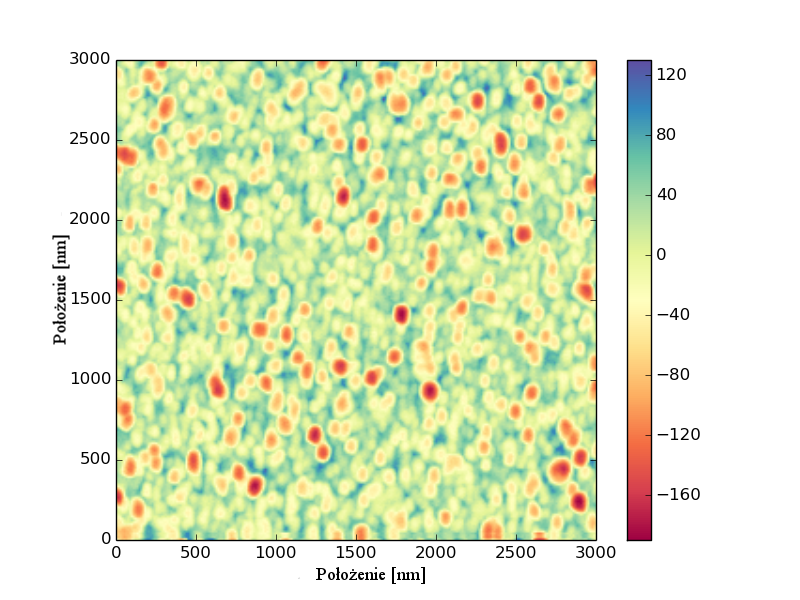
\includegraphics[width=\textwidth]{images/multilayer/ag30nm-afm-measure.png}
		\caption{Pomiary grubości na powierzchni napylonej warstwy $30$~nm srebra za pomocą AFM. Pomiary wykonał dr~Tomasz~Stefaniuk.} 
		\label{fig:ag30nm-afmmeasure}
\end{figure}


Efektywne współczynniki przenikalności elektrycznej uzyskiwane za pomocą wzoru~(\ref{eq:effmedium}) w~znacznym stopniu zmieniają się w~wyniku wprowadzenia chropowatości~\cite{ludwig2012impact}. Szczególnie dużą zmienność można zaobserwować w~okolicach rezonansu dla $\varepsilon_{z}$, czyli~w zakresie długości fali, dla którego projektowane są własności metamateriału. Zbliżenie wartości do przewidywanych w~warunkach homogenizacji można zaobserwować w~przypadku struktur, dla których punkty odpowiadające pomiarom grubości z~mikroskopu są bardziej oddalone - próbkowanie pomiaru mikroskopowego jest rzadsze niż w~symulacji numerycznej. Ze względu na przybliżenie granicy warstwy pomiędzy punktami pomiarowymi z~AFM poprzez funkcję gładką, Ludwig i~inni otrzymują większe gładkie obszary na powierzchni symulowanej granicy między ośrodkami~\cite{ludwig2012impact}. 

\begin{figure}[!hbt]
	\begin{center}
	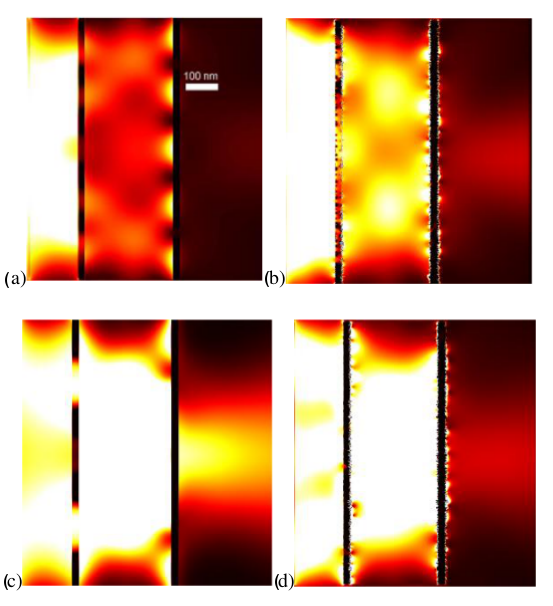
\includegraphics[width=.9\textwidth]{images/multilayer/plp-chropo.png}
	\end{center}
	\caption{Rozkład natężenia pola elektromagnetycznego wewnątrz i~poza strukturą warstwową o~własnościach supersoczewki z~warstwami gładkimi- (a) i (c) oraz chropowatymi- (b) i (d), oświetlonej za pomocą źródła monochromatycznego o~długościach fali odpowiednio (a),(b)~$\lambda=430$~nm  i~(c),(d) $\lambda=490$~nm~\cite{Stolarek_2013}}
	\label{fig:plp-chropo-fdtd}
\end{figure}

Nierówność warstw może mieć pozytywny wpływ na niektóre parametry opisujące zdolności obrazujące wielowarstwy. Uwzględnienie chropowatości może zwiększyć współczynnik transmisji przez granicę dwóch ośrodków poprzez skrócenie zasięgu propagacji plazmonów powierzchniowych w~przypadku przypadkowej chropowatości oraz dodatkowe wzmocnienie fal ewanescentnych za pomocą sinusoidalnej chropowatości o~okresie podfalowym~\cite{huang2012subwavelength}. Przykład układu dla którego wprowadzenie chropowatości zwiększa współczynnik transmisji dla wąskiego zakresu długości fal, przedstawia rozkład pola elektromagnetycznego na rysunku \ref{fig:plp-chropo-fdtd}~a~-~b. W ogólności jednak wzrost chropowatości powierzchni zmniejsza współczynnik transmisji przez strukturę warstwową, co możemy zaobserwować po zmianie długości fali oświetlającej soczewkę na rozkładach pola na rysunkach \ref{fig:plp-chropo-fdtd}~c~i~d. 

\begin{figure}[htb]
		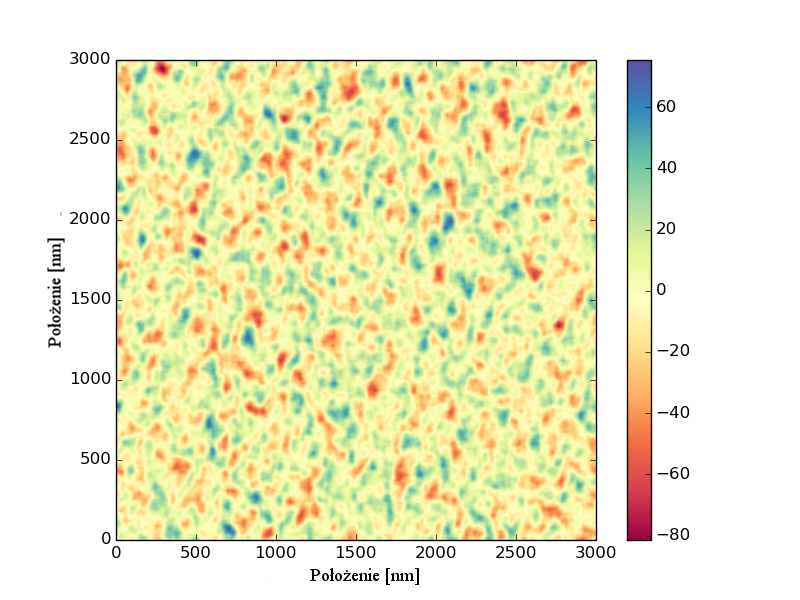
\includegraphics[width=\textwidth]{images/multilayer/ag30nm-afm-generated.png}
		\caption{Wizualizacja powierzchni chropowatej wygenerowanej na podstawie pomiarów AFM. Generowana dwuwymiarowa macierz losowa podlegające rozkładowi normalnemu o~widmowej gęstości mocy odpowiadającej wynikom pomiarów za pomocą AFM.} 
		\label{fig:ag30nm-afmgene}
%	Generator:
%	pomocnicze/wielowarstw/chropo/gen-chropo.py
\end{figure}


Zmiana właściwości materiałów, z~których zbudowana jest wielowarstwa, na charakteryzujące się mniejszą absorpcją, nie może być wykorzystana do kompensacji strat transmisji w~wyniku nierówności warstw. Wprowadzenie chropowatości prowadzi do powstania losowych zaburzeń rozkładu pola elektromagnetycznego, których interferencja wprowadza zniekształcenie optycznej funkcji przenoszenia~(ang.~OTF - Optical Transfer Function)~\cite{citeulike:2926459}. Odpowiednio dobrany współczynnik absorpcji wewnątrz metali zapewnia szybkie zanikanie losowych zaburzeń umożliwiając zachowanie płaskiego charakteru OTF~\footnote{Płaski charakter OTF oznacza równomierne tłumienie wszystkich częstości przestrzennych. Jest to równoważne z małą szerokością PSF, a tym samym wysoką rozdzielczością obrazowania}. Szczególne znaczenie dla zachowania własności obrazowania podfalowego ma płaszczyzna wyjściowa wielowarstwy, na której utrzymanie RMS poniżej $0.6$~nm jest kluczowe dla uzyskania PSF o~szerokości podfalowej~\cite{guo2014negative}.

Należy zwrócić uwagę, że na skutek chropowatości współczynnik $\varepsilon_z$ zostaje zmniejszony w~okolicach rezonansu~\cite{guo2014negative} (dla idealnej supersoczewki $\varepsilon_{z} \to - \infty$), co powoduje, że możliwa jest efektywna transmisja wyższych częstości przestrzennych, a co za tym idzie zwiększenie zdolności rozdzielczej układu. Własności obrazujące, które są optymalne przy płaskim kształcie OTF zostają jednocześnie zaburzone, a ich zachowanie możliwe jest poprzez użycie materiałów o~większym współczynniku absorpcji. Na podstawie takiego rozważania Zhen Guo i~in.~\cite{guo2014negative} wnioskują, że chropowatość w~zasadniczy sposób pogarsza zdolności obrazujące supersoczewki. Zdolność rozdzielcza jest natomiast determinowana poprzez stratność użytych materiałów.

\begin{figure}[htb]
	\centering
	\begin{subfigure}[b]{.45\textwidth}
		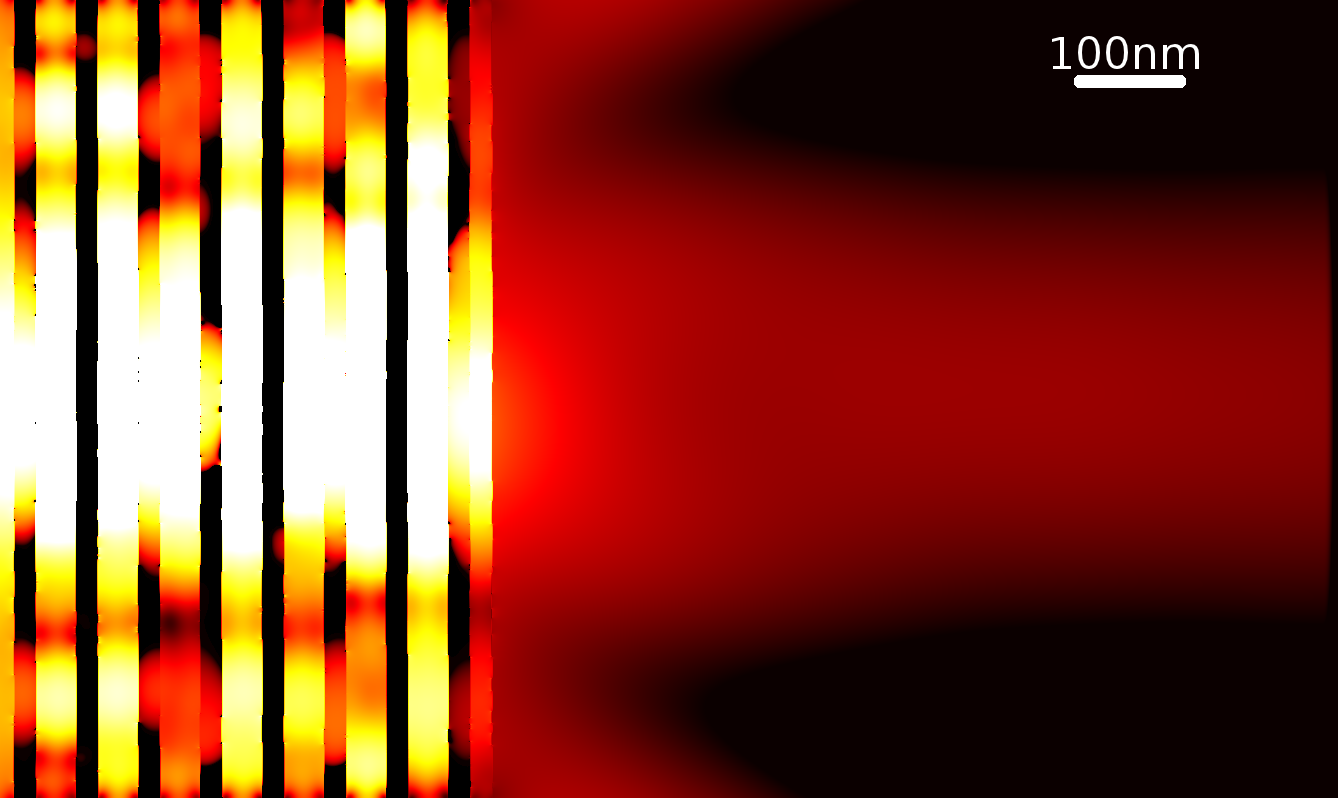
\includegraphics[width=\textwidth]{images/multilayer/oer-rms01.png}
		\caption{$RMS=0.1$~nm}
	\end{subfigure}
	\begin{subfigure}[b]{.45\textwidth}
		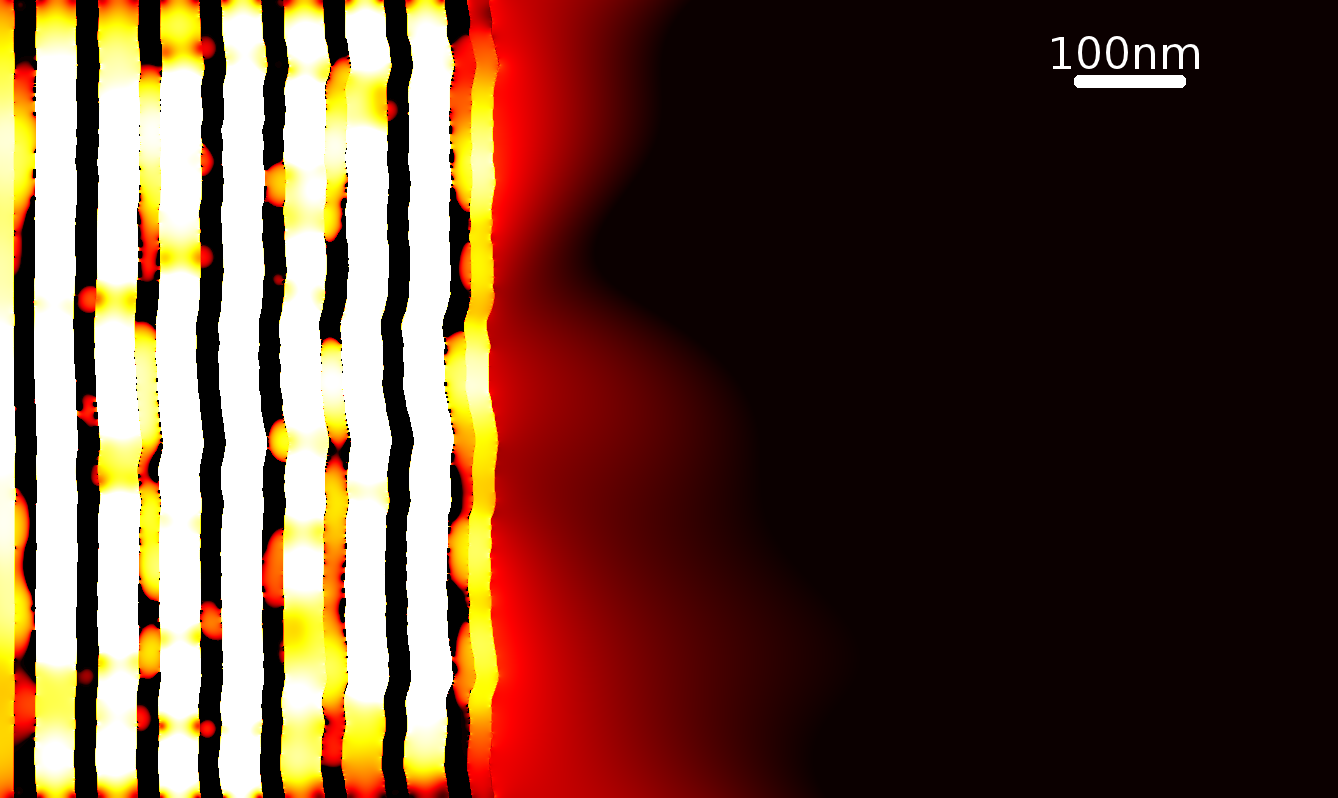
\includegraphics[width=\textwidth]{images/multilayer/oer-rms05.png}
		\caption{$RMS=0.5$~nm}
	\end{subfigure}
	\caption{Wyniki symulacji wielowarstwy o~17 chropowatych granicach ośrodków, z~różnymi wartościami RMS charakteryzującymi chropowatość warstw. Na ilustracji (b) obserwujemy znaczne ograniczenie długości wektora Poyntinga fali E-M propagującego się w~pole dalekie na skutek interferencji wielu fal płaskich losowo zaburzonych przez nierówności~\cite{pastuszczak2013engineering}.}
	\label{fig:rmsem}
	
\end{figure}

Porównanie wyników prac numerycznych prowadzonych przez różnych autorów dotyczących wpływu chropowatości na współczynnik transmisji, szerokość i~kształt funkcji rozmycia punktu~(ang. PSF~-~point spread function) oraz na zdolność rozdzielczą wielowarstwy wymaga uwzględnienia różnic w~zastosowanej przez nich metodyce. Kluczowym elementem jest sposób generacji powierzchni chropowatej - w~niektórych pracach nie jest uwzględniana autokorelacja nierówności~\cite{guo2014negative}, przez co zaniedbane zostają charakterystyczne elementy topologii widoczne w~pomiarach za pomocą AFM. W innych wykorzystywane są algorytmy heurystyczne, łączące punkty z~pomiarów mikroskopowych za pomocą wielomianów sklejanych\footnote{tzw. krzywa B-sklejana, w~literaturze polskiej postulowana bywa również nazwa splajn od angielskigo B-spline}~\cite{ludwig2012impact}, w~innych pracach autorzy opierają się na widmowym rozkładzie gęstości mocy zmiennej losowej~\cite{pastuszczak2013engineering}. Przykład powierzchni chropowatej wygenerowanej na podstawie pomiarów z~mikroskopu AFM z~wykorzystaniem ostatniej z~wymienionych metod znajduje się na ilustracji~\ref{fig:ag30nm-afmgene}.

Niezależnie od zastosowanej metodyki symulacji pola elektromagnetycznego i~generacji warstw chropowatych składających się na supersoczewki zbudowane ze struktur MDM, wyniki pozwalają na wysunięcie zgodnych wniosków. Uzyskanie nadrozdzielczego obrazowania przez omawiane układy  możliwe jest jedynie w~wielowarstwach o~RMS$<1.5$~nm~\citep{guo2014negative,stefaniuk2011effect,ludwig2012impact}. Ponieważ każda chropowata powierzchnia przyczynia się do rozproszenia fali -  ze wzrostem liczby warstw własności transmisyjne i~obrazujące stosu MDM stają się bardziej wrażliwe na chropowatości powierzchni \cite{guo2014negative}. W przypadku stosów składających się z~kilkunastu warstw, RMS nawet na poziomie $0.5$~nm może uniemożliwić uzyskanie wysokiego współczynnika transmisji, a co za tym idzie praktycznego wykorzystania tego typu soczewek~\cite{pastuszczak2013engineering}. Wpływ chropowatości na rozkład pola E-M jak i~współczynnik transmisji przez stos metaliczno-dielektryczny prezentują rozkłady pola E-M na rysunku~\ref{fig:rmsem}.




%%%%%%%%Obrazki z~publikacji w~PLP - wyniki pomoarow afm w~1d i~2d
%%%%%%%%\begin{figure}[htb]
%%%%%%%%		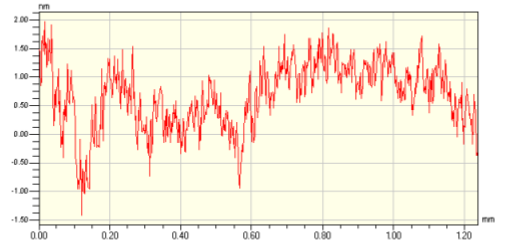
\includegraphics[width=\textwidth]{images/multilayer/plp-afm-chropo-1d.png}\\
%%%%%%%%\end{figure}

%%%%%%%%\begin{figure}[htb]
%%%%%%%%		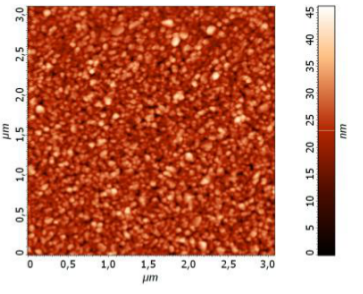
\includegraphics[width=\textwidth]{images/multilayer/plp-afm-chropo.png}\\
%%%%%%%%\end{figure}



